\documentclass[a4paper,12pt]{article}
\usepackage[utf8]{inputenc}
\usepackage[spanish]{babel}
\usepackage{graphicx}
\usepackage{amsmath}
\usepackage{amsfonts}
\usepackage{amssymb}
\usepackage{hyperref}
\usepackage{float}
\usepackage[numbers]{natbib}
\usepackage{multicol}



% Configuración de márgenes
\usepackage[left=3cm,right=3cm,top=2.5cm,bottom=2.5cm]{geometry}

% Títulos y subtítulos en formato moderno
\usepackage{titlesec}
\titleformat{\section}{\large\bfseries}{\thesection}{1em}{}
\titleformat{\subsection}{\normalsize\bfseries}{\thesubsection}{1em}{}

% Información del documento
\title{Proyecto de IA-Simulaci\'on\\\textit{Tema: Movilidad Humana en La Habana}}
\author{Yoan Ren\'e Ramos Corrales  C-412  \and  David Cabrera Garc\'ia  C-411}



\begin{document}

% Título
\maketitle

% Abstract en inglés
\renewcommand{\abstractname}{Abstract}
\begin{abstract}
This project proposal for the Artificial Intelligence and Simulation courses aims to develop a mobility trajectory generator for Havana. The generator will simulate the movement of the city's inhabitants, focusing primarily on the bus networks. The primary goal is to estimate the number of residents present in each municipality of the capital over the course of a 24-hour day.

\end{abstract}
% Palabras clave en inglés
\textbf{Keywords:} agent-based system, BDI, discrete-event simulation
% Abstract
\renewcommand{\abstractname}{Resumen}
\begin{abstract}
Esta propuesta de proyecto para las asignaturas de Inteligencia Artificial y Simulación tiene como objetivo desarrollar un generador de trayectorias de movilidad para La Habana. El generador simulará el movimiento de los habitantes de la capital, considerando principalmente las redes de ómnibus. El objetivo principal es estimar la cantidad de habitantes que se encuentran en cada municipio de la capital durante las 24 horas de un día.
\end{abstract}
% Palabras clave en español
\textbf{Palabras clave:} sistema basado en agentes, BDI, simulación por eventos discretos

\newpage
\tableofcontents
\newpage
% Sección de Introducción
\section{Introducción}
Los estudios sobre la movilidad humana se enfocan en describir cómo las personas se desplazan dentro de un sistema o red. El análisis y la predicción de estos movimientos tienen aplicaciones en diversas áreas, como la propagación de enfermedades, la planificación urbana, la ingeniería del tráfico y los mercados financieros, entre otras. En el caso de enfermedades infecciosas como la COVID-19, se sabe que la movilidad humana es un factor clave para su propagación.

Actualmente, se recopila una enorme cantidad de datos sobre trayectorias de movilidad a través de sensores y diversas aplicaciones. Sin embargo, su uso directo presenta desafíos debido a preocupaciones sobre la privacidad, consideraciones comerciales, datos faltantes y altos costos de implementación. Por este motivo, la generación de datos sintéticos de trayectorias de movilidad ha surgido como una tendencia emergente para mitigar las dificultades asociadas al uso de datos reales. La investigación en la generación de trayectorias sintéticas está ganando gran atención, como lo demuestra el creciente número de publicaciones en este campo interdisciplinario.

Atendiendo a lo anterior se propone entonces la creaci\'on de un modelo capaz de simular el movimiento de los habitantes de la La Habana considerando principalmente las redes de \'omnibus de la capital. 

% Sección de Metodología
\section{Metodología}
\subsection{Preliminares}
Nuestra simulación se basa en un \textbf{modelo de eventos discretos}, que captura los cambios de estado en momentos específicos del tiempo \cite{law2014simulation}. El sistema está diseñado bajo un enfoque de \textbf{sistemas basados en agentes} \cite{wooldridge2009introduction}, donde el \textbf{medio ambiente} es la red de transporte público de La Habana, y los \textbf{agentes} son pasajeros que interactúan con dicho medio.

\subsection{Definci\'on del Medio Ambiente}
\label{medio_ambiente}

El medio ambiente en el que operan los agentes está sobre un \textbf{multigrafo} $G = (V, E, \rho, w)$ que modela la red de transporte público de La Habana \cite{evans2021public}. El multigrafo se define de la siguiente manera:

\begin{itemize}
    \item $V = \{v_1, v_2, \dots, v_n\}$ es el conjunto de vértices que representan las \textbf{paradas de transporte público}.
    \item $E = \{e_1, e_2, \dots, e_m\}$ es el conjunto de aristas, donde cada arista $e \in E$ representa una \textbf{conexión directa} entre dos paradas a través de una ruta específica.
    \item $\rho: E \rightarrow R$ es una función que asigna a cada arista una ruta específica $\rho_i \in R$, donde $R$ es el conjunto de rutas disponibles en la red de transporte.
    \item $w: E \rightarrow \mathbb{R}^+$ es una función de peso que asigna una distancia a cada arista, representando la \textbf{distancia} entre las paradas por una ruta específica.
\end{itemize}.

\subsubsection{Características del Medio Ambiente}

\begin{itemize}
    \item \textbf{Desplazamiento de las guaguas}: Las guaguas se desplazan a lo largo del multigrafo $G$, siguiendo rutas predefinidas. Cada guagua sigue una ruta asignada $\rho_i \in R$, que corresponde a un conjunto de aristas en el multigrafo que conectan varias paradas, pero no actúan como agentes autónomos en la simulación.
    
    \[
    \text{Ruta de la guagua } i: \rho_i = (v_{i1}, v_{i2}, \dots, v_{ik})
    \]
    
    Donde $v_{i1}, v_{i2}, \dots, v_{ik} \in V$ son las paradas consecutivas en la ruta $\rho_i$.
    
    \item \textbf{Paradas y municipios}: Cada parada $v \in V$ pertenece a un municipio específico de La Habana. Formalmente, existe una función $\mu: V \rightarrow M$, donde $M$ es el conjunto de municipios, y $\mu(v)$ asigna un municipio a cada parada $v$. Esto permite modelar la distribución geográfica de las paradas dentro de la ciudad y analizar las rutas dentro de cada municipio o entre diferentes municipios.
    
    \item \textbf{Movilidad y tiempos de desplazamiento}: Cada guagua tiene un tiempo de desplazamiento asociado a cada arista $e_\ell^{ij} \in E_{ij}$ en su ruta, que está determinado por la función de peso $w(e_\ell^{ij})$, la cual representa la \textbf{distancia} entre las paradas $v_i$ y $v_j$ en una ruta específica.
    
    \item \textbf{Frecuencia de las guaguas}: Cada ruta $\rho_i$ tiene un intervalo de tiempo $\tau_i$ que representa la frecuencia con la que las guaguas parten de la primera parada $v_{i1}$. Este parámetro es esencial para simular la disponibilidad de transporte en diferentes rutas.

    \item \textbf{Accesibilidad entre paradas}: Para cada agente, es posible llegar desde cualquier parada $v_i \in V$ a cualquier otra parada $v_j \in V$ mediante una o más rutas, ya sea de forma directa o a través de transbordos. Esta propiedad garantiza que la red de transporte cubre toda la ciudad y que los pasajeros pueden llegar a sus destinos, incluso si deben cambiar de guagua en varias ocasiones.
    
    \item \textbf{Agentes pasajeros}: Los pasajeros son los agentes del sistema y toman decisiones sobre qué ruta tomar para llegar a su destino. Estas decisiones dependen del estado del multigrafo (disponibilidad de guaguas, tiempos de espera, distancias entre paradas, etc.).

    \item \textbf{Interacción dinámica}: Los pasajeros interactúan dinámicamente con el multigrafo $G$. Deciden abordar una guagua en una parada $v_i$ dependiendo de la ruta que ésta sigue, la distancia a su destino y el tiempo de espera. A medida que las guaguas se desplazan por las aristas, cambian el estado del entorno, lo cual afecta las decisiones de los pasajeros.
    
    \item \textbf{Actualización del estado}: El estado del multigrafo $G$ y de los agentes pasajeros se actualiza continuamente en función de la posición de las guaguas en las rutas, los tiempos de desplazamiento y la disponibilidad de conexiones en cada parada.
\end{itemize}


\subsection{Definición del Agente}
\label{sec:defagente}

Cada agente en la simulación está basado en la arquitectura \textbf{BDI (\textit{Belief-Desire-Intention})} \cite{rao1995bdi}, donde un agente tiene la capacidad de planificar rutas, tomar decisiones y ajustar su comportamiento según las circunstancias del entorno. Formalmente, el agente $A$ se define por los siguientes componentes:

\subsubsection{Creencias (Beliefs)}

El agente mantiene una serie de creencias $\mathcal{B}$ que definen su percepción del entorno y de sí mismo. Estas creencias se modelan como un conjunto de variables de estado:

\begin{itemize}
    \item $\mathcal{B}.\text{parada\_origen}$: La parada de transporte público en la que el agente comenzó su viaje.
    \item $\mathcal{B}.\text{parada\_actual}$: La parada donde el agente se encuentra actualmente.
    \item $\mathcal{B}.\text{destino}$: La parada de destino del agente.
    \item $\mathcal{B}.\text{paradas\_next}$: Lista de paradas donde el agente debe cambiar de vehículo en su ruta planificada.
    \item $\mathcal{B}.\text{current\_time}$: El tiempo actual en la simulación.
    \item $\mathcal{B}.\text{ruta\_planificada}$: La ruta que el agente ha planificado para llegar a su destino.
    \item $\mathcal{B}.\text{llego\_trabajo}$: Booleano que indica si el agente ha llegado a su lugar de trabajo.
    \item $\mathcal{B}.\text{regreso\_casa}$: Booleano que indica si el agente ha regresado a su casa.
    \item $\mathcal{B}.\text{cogio\_carro}$: Booleano que indica si el agente ha decidido utilizar un automóvil privado en lugar del transporte público.
    \item $\mathcal{B}.\text{caminando}$: Booleano que indica si el agente ha decidido caminar hacia su destino.
\end{itemize}

\subsubsection{Deseos (Desires)}

Los deseos $\mathcal{D}$ del agente son los objetivos que quiere lograr, y pueden ser dinámicos a lo largo del tiempo. En este modelo, los deseos más relevantes son:

\begin{itemize}
    \item $\mathcal{D}.\text{llegar\_destino}$: El agente desea llegar a su destino.
    \item $\mathcal{D}.\text{regresar\_casa}$: El agente desea regresar a su casa.
\end{itemize}

\subsubsection{Intenciones (Intentions)}

Las intenciones $\mathcal{I}$ del agente son los planes concretos que ejecuta para cumplir sus deseos, dadas sus creencias actuales. Por ejemplo:

\begin{itemize}
    \item $\mathcal{I}.\text{salir\_de\_casa}$: El agente decide salir de su casa para comenzar su viaje.
    \item $\mathcal{I}.\text{esperar\_guagua}$: El agente decide esperar una guagua (autobús) en la parada actual.
    \item $\mathcal{I}.\text{caminar}$: El agente decide caminar hacia su destino si no hay una guagua disponible despu\'es de un tiempo o si es una opción más conveniente según sus preferencias.
    \item $\mathcal{I}.\text{coger\_carro}$: El agente decide utilizar un automóvil privado si la espera en la parada es muy larga o si es más beneficioso.
\end{itemize}

\subsubsection{Preferencias}

Cada agente tiene un conjunto de preferencias $\mathcal{P}$ que influencian la toma de decisiones. Estas preferencias varían entre agentes y son modeladas como valores aleatorios entre 0 y 1, ponderando diferentes factores en la toma de decisiones. Las preferencias principales son:

\begin{itemize}
    \item $\mathcal{P}.\text{rapidez}$: Preferencia por rutas rápidas.
    \item $\mathcal{P}.\text{comodidad}$: Preferencia por rutas cómodas (menor número de paradas y cambios de guagua).
    \item $\mathcal{P}.\text{ganancias}$: Preferencia por poder pagar un autom\'ovil privado.
    \item $\mathcal{P}.\text{laboriosidad}$: Preferencia por llegar al trabajo.
    \item $\mathcal{P}.\text{condicion\_fisica}$: Nivel de condición física que afecta la velocidad al caminar o el tiempo máximo que puede soportar antes de decidir tomar un vehículo.
    \item $\mathcal{P}.\text{paciencia}$: Tolerancia a las esperas prolongadas en la parada. Si se impacienta, el agente podría cambiar sus intenciones y optar por otras rutas o modos de transporte.
\end{itemize}

\subsubsection{Decisiones del Agente}

El agente toma decisiones basadas en sus creencias, deseos e intenciones. Estas decisiones incluyen:

\begin{itemize}
    \item \textbf{Elección de Ruta:} El agente utiliza un algoritmo de búsqueda A* para planificar su ruta en el multigrafo que representa la red de transporte público \cite{hart1968formal}. Esta ruta se ajusta dinámicamente según sus preferencias y el estado actual del sistema (como la disponibilidad de guaguas y la congestión).
    
    \item \textbf{Cambio de Ruta:} Si el agente considera que una ruta alternativa es más favorable (por ejemplo, si una guagua diferente llega a la parada), puede recalcular su ruta usando A* con diferentes estrategias \cite{hart1968formal}, como minimizar la distancia o reducir el número de paradas.

    \item \textbf{Impaciencia y Abandono de la Parada:} Si el agente lleva demasiado tiempo esperando una guagua, se pude impacientar. En este caso, el agente puede decidir abandonar la parada y caminar o coger un carro hacia su destino. El tiempo de espera antes de abandonar la parada se calcula en función de su preferencia de paciencia.
\end{itemize}
\subsection{Simulación por Eventos Discretos}
La simulación desarrollada sigue un enfoque de eventos discretos, en el cual las interacciones de los agentes con el entorno se modelan en función de la ocurrencia de eventos programados en el tiempo. A continuación, se detallan los aspectos clave de este enfoque y cómo los agentes interactúan con el sistema de transporte simulado.

\subsubsection{Manejo de Eventos}
La simulación se organiza en torno a una cola de prioridad (\textit{heap}) de eventos \cite{cormen2009introduction}. Cada evento contiene una marca temporal y un conjunto de argumentos que describen la acción a realizar. Los tipos principales de eventos incluyen:
\begin{itemize}
    \item \textbf{Llegada de Agente a Parada:} Un agente alcanza una parada y elige su próximo curso de acción, ya sea subirse a una guagua, continuar caminando, o esperar.
    \item \textbf{Inicialización de Guagua:} Una guagua comienza su recorrido por una ruta específica según la frecuencia de su ruta.
    \item \textbf{Movimiento de Guagua:} La guagua avanza de una parada a la siguiente, permitiendo que los pasajeros suban y bajen.
\end{itemize}

\subsubsection{Interacción de los Agentes con el Entorno}
En cada evento, los agentes actualizan sus creencias e intenciones basándose en la información disponible en el entorno tal como se describe en la secci\'on \ref{sec:defagente}.

\subsubsection{Eventos Clave en la Simulación}
El flujo de la simulación depende del desencadenamiento de los eventos y las decisiones de los agentes. Los eventos se procesan en orden cronológico, lo que permite que la simulación avance de manera dinámica. El entorno, representado por un grafo de conexiones de rutas de guaguas, proporciona el contexto para las acciones de los agentes. La interacción de los agentes con este grafo y con las guaguas es fundamental para el éxito de sus trayectorias.

A medida que los agentes completan sus trayectos o regresan a sus puntos de origen, el sistema de eventos sigue generando nuevas acciones, asegurando que la simulación capture la complejidad de la movilidad en un entorno urbano dinámico.

\subsection{Uso de Modelos de Lenguaje para la Configuración y Ejecución de la Simulaci\'on}

En el desarrollo de la simulación de movilidad humana para la ciudad de La Habana, se ha implementado un enfoque que integra modelos de lenguaje avanzados (LLMs, por sus siglas en inglés) para automatizar tanto la configuración como la ejecución de la simulación \cite{llm_overview}. Este enfoque permite a los usuarios interactuar con el sistema mediante lenguaje natural, facilitando el proceso de configuración y la posterior interpretación de los resultados generados por la simulación.

\subsubsection{Generación y Ejecución de la Simulación}

El modelo de lenguaje utilizado, \textit{Gemini-1.5 Flash} \cite{gemini_model}, ha sido integrado al sistema mediante una API, permitiendo que, a partir de una entrada textual del usuario, se genere un archivo de configuración en formato JSON que contiene los parámetros clave para la simulación. Estos parámetros incluyen:

\begin{itemize}
    \item Cantidad de ómnibus.
    \item Tiempo total de simulación.
    \item Número de agentes.
    \item Archivos de distribución de población y trabajos por municipio.
    \item Frecuencias de salida de las rutas de transporte.
    \item Probabilidades de retorno a los hogares.
    \item Intervalos de partida de los agentes.
\end{itemize}

Tras la generación del archivo JSON, el sistema procede a ejecutar automáticamente la simulación utilizando los parámetros establecidos por el modelo de lenguaje. La ejecución se realiza sin intervención adicional del usuario, permitiendo que el proceso sea ágil y eficiente.

\subsubsection{Análisis de los Resultados}

Al finalizar la simulación, el LLM no solo proporciona los resultados brutos generados, sino que además realiza un análisis detallado de los mismos. Los resultados de la simulación, que se guardan en archivos CSV, son procesados y formateados para su presentación de manera comprensible. A través del modelo de lenguaje, el usuario puede recibir un análisis estadístico completo de los datos, acompañado de gráficos generados automáticamente para facilitar la visualización de las dinámicas de movilidad. Estos gráficos incluyen la distribución de personas por municipio a lo largo del día, reflejando el impacto de las diferentes configuraciones de transporte y comportamiento de los agentes.

Un ejemplo típico de interacción con el LLM puede incluir preguntas como: \textit{“¿Qué sucede si solo está disponible la ruta P11?”} o \textit{“¿Cómo afectaría a la población de Habana del Este la falta de guaguas en la ruta P1?”}. El LLM ajusta los parámetros de la simulación según la consulta, ejecuta la simulación y presenta un análisis exhaustivo de los resultados, considerando las condiciones impuestas por el usuario.

\subsubsection{Ventajas del Uso de LLMs en la Simulación}
\begin{itemize}
    \item Automatización integral del proceso de configuración, ejecución y análisis de simulaciones.
    \item Reducción significativa de la complejidad para los usuarios, permitiendo interactuar mediante lenguaje natural sin necesidad de conocimientos técnicos detallados.
    \item Capacidad de personalizar dinámicamente la simulación en respuesta a preguntas o hipótesis específicas planteadas por el usuario.
    \item Generación automática de informes estadísticos y gráficos que facilitan la interpretación de los resultados.
\end{itemize}




% Sección de Resultados
\section{Resultados y Discusi\'on}

\subsection{Introducción}

Se presentan los resultados de una serie de simulaciones realizadas para analizar el comportamiento de diferentes parámetros y su impacto en el rendimiento del sistema de transporte público en La Habana. Se simularon diferentes escenarios para evaluar el impacto de la capacidad del autobús, el número de agentes y la existencia de rutas en la eficiencia del transporte público. En la simulaci\'on el conjunto $R$ de la secci\'on \ref{medio_ambiente}  utilizado fue $\{P1,P2,...,P16,PC\}$ conocidas por todos los cubanos como los \textit{pe}, las cuales son las rutas prinicipales del transporte en La Habana, luego las componentes modeladas (paradas, conexiones entre paradas, etc.) son las definidas por dichas rutas. Con respecto a la distribuci\'on de datos utilizada se apoya en la Tabla: \textit{Poblaci\'on de Cuba por provincias y municipios} para la proporci\'on de los capitalinos por sus respectivos municipios \cite{onei2022}, y en la Tabla: \textit{La Habana: Distribuci\'on de los ocupados seg\'un municipios de residencia y municipios donde radican las entidades \%} para determinar qu\'e porcentaje de personas de un municipio $M_i$ trabajan en un municipio $M_j$ \cite{aja2023}.  Adem\'as se tuvo en cuenta los horarios \textit{pico}, en que las personas salen a su lugar de trabajo y regresan de este, los cuales se consider\'o que son de 6:00am a 8:00am y de 3:00pm a 5:00pm. Con respecto a las paradas y rutas se utiliz\'o la base de datos de  la app MWurbanos \cite{apklis}. Todas las gr\'aficas y tablas plasmadas en este documento se puden consultar en una mayor escala \href{https://github.com/YoanRene/AI-Sim/tree/master/docs/imgs}{aqu\'i}. 

\subsection{Parámetros de la Simulación}

Los siguientes parámetros se utilizaron en las simulaciones:

\begin{itemize}
\item Número de agentes: Determina la cantidad de personas que requieren transporte. Se prob\'o con 50, 500, 1000 y 5000.
\item Capacidad del autobús: Define la cantidad máxima de pasajeros que puede transportar un autobús. Se prob\'o con 2, 5,10 y 20.
\item Ruta inexistente: Eliminamos una ruta que existe en la realidad para evaluar el impacto en la distribución de pasajeros. Se prob\'o con la ausencia de todos los \textit{pe}.
\end{itemize}

\subsection{Resumen de las Métricas Clave}

Se evaluaron las siguientes métricas en cada simulación de un total de 69:

\begin{itemize}
\item Viajes completados: La mayoría de las simulaciones lograron un alto porcentaje de viajes completados por agentes, con un promedio general de 93.4\%.
\item Destinos completados: Se observa una alta correlación entre viajes completados y destinos completados por agentes donde este \'utimo representa tanto la ida al trabajo como el regreso, con un promedio de 93.3\%.
\item Tiempo promedio de viaje al trabajo del agente: El tiempo promedio de viaje varía significativamente entre las diferentes configuraciones de la simulación, con un promedio general de 139.5 minutos, lo que equivale a 2 horas y 19 minutos aproximadamente, bastante cerca de la realidad cubana.
\item Porcentaje de Llenado: Este valor representa la cantidad de personas que una guagua lleva en promedio por cada parada, este fue de 19.5\%, lo cual es bastante bajo para la situaci\'on actual en la capital, en parte se debe a los horarios  nocturnos; no obstante hay espacio de mejora en la simulaci\'on para un valor m\'as real de esta m\'etrica.
\end{itemize}

\subsection{Resultados}
El objetivo fundamental de este proyecto siempre fue determinar para una hora espec\'ifica la cantidad de personas que hay en un municipio, esto se logra tal como se muestra en el ejemplo de la Figura \ref{fig:1} para una simulaci\'on dada (aclarar que no se observan todos los municipios por un tema de extensi\'on de la tabla).

\begin{figure}[H]
    \centering
    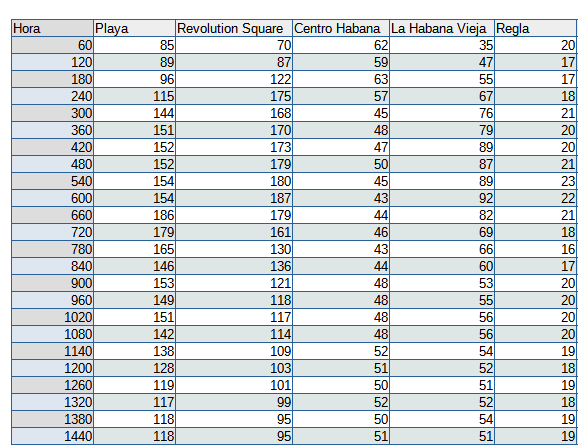
\includegraphics[width=0.8\textwidth]{imgs/s1000.png}
    \caption{Cantidad de agentes en un horario(minutos a partir de las 6:00am) en un municipio dado}
    \label{fig:1}
\end{figure}

Por la cantidad significativa de valores expresados se determinaron dos formas distintas de expresar el objetivo central del proyecto sin que duela la vista de tantos n\'umeros, aunque quiz\'as esforzando un poco m\'as la vista por el tamaño de las gráficas, no obstanste se reitera revisar con más detalle \href{https://github.com/YoanRene/AI-Sim/tree/master/docs/imgs}{aqu\'i}, una de estas dos formas de expresar lo mismo se encuentra en la Figura \ref{fig:2}, en la que se pude notar dos curvas que sobresalen del resto en horario laboral, las cuales representan al municipio Playa y Plaza de la Revoluci\'on, esto se debe principalmente a la gran cantidad de empleos que existen en estas localidades.

\begin{figure}[H]
    \hspace{-3cm}
    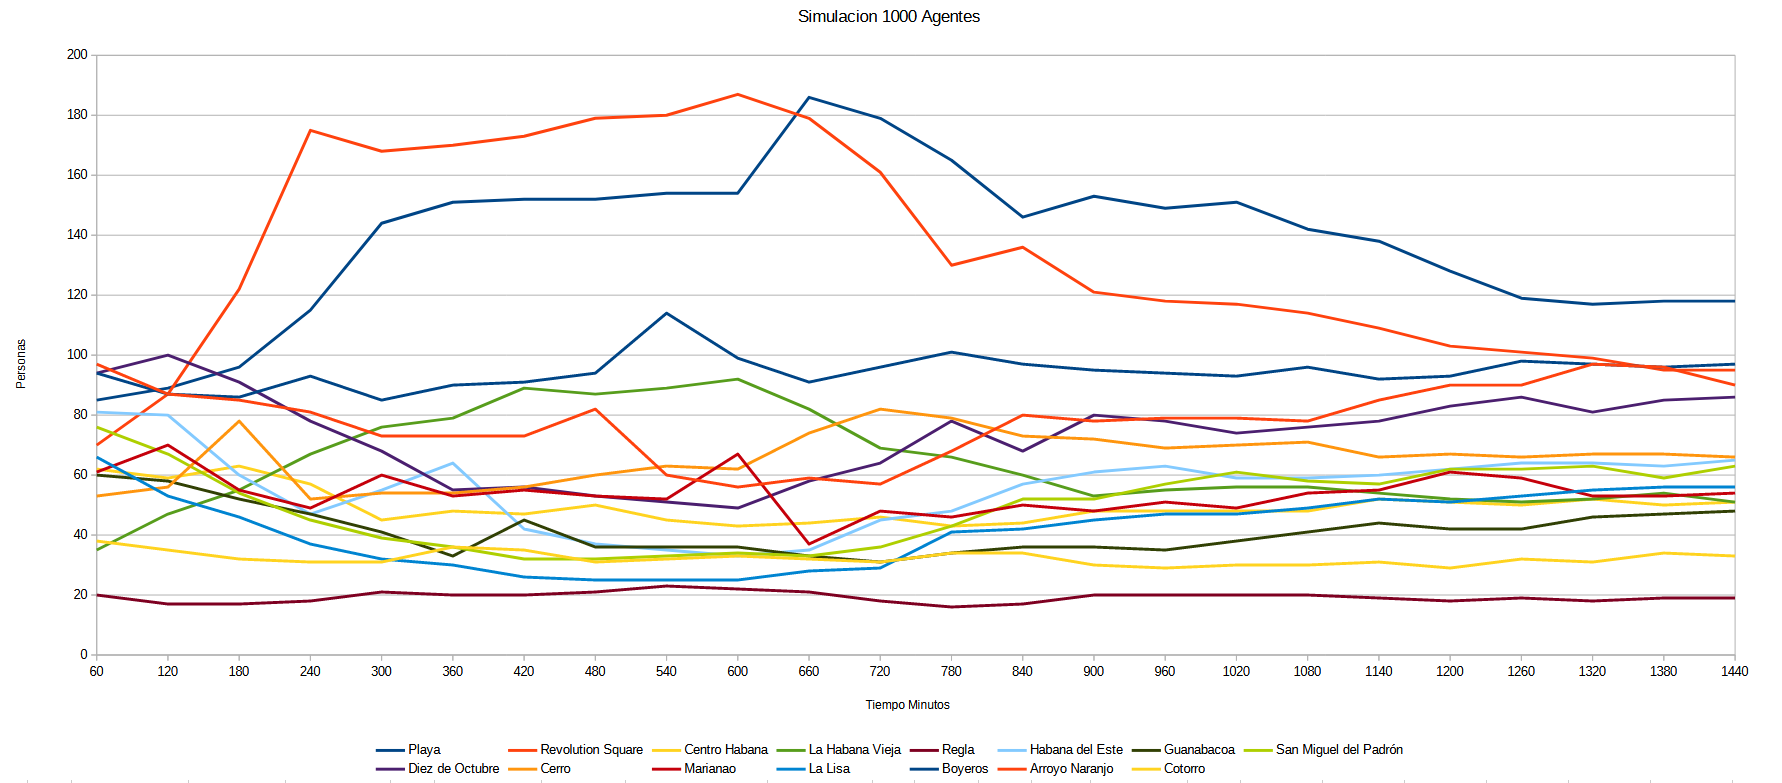
\includegraphics[width=1.4\textwidth]{imgs/s1000c20.png}
    \caption{Cantidad de agentes vs Tiempo Minutos (Simulaci\'on 1000 agentes con capacidad de las guaguas de 20, y sin la ausencia de rutas)}
    \label{fig:2}
\end{figure}

La otra forma en que expresamos lo mismo es a través de un mapa de calor de La Habana, lo cual entre más intenso el color de un municpio en una hora determinada más cantidad de agentes hay en este, para representar esto se hizo una pequeña interfaz visual en la que dada una simulación se es capaz de escoger la hora, y observar el mapa de calor correspondiente tal como se aprecia en la Figura \ref{fig:3}, como dato interesante en el desarrollo de la interfaz se utilizó una archivo \textit{geojson} desarrollado por un importante miembro de la facultad de MATCOM de la UH; para los curiosos puden consultar \href{https://github.com/yudivian/cuba-geojsons}{aqu\'i} .

\begin{figure}[H]
    \centering
    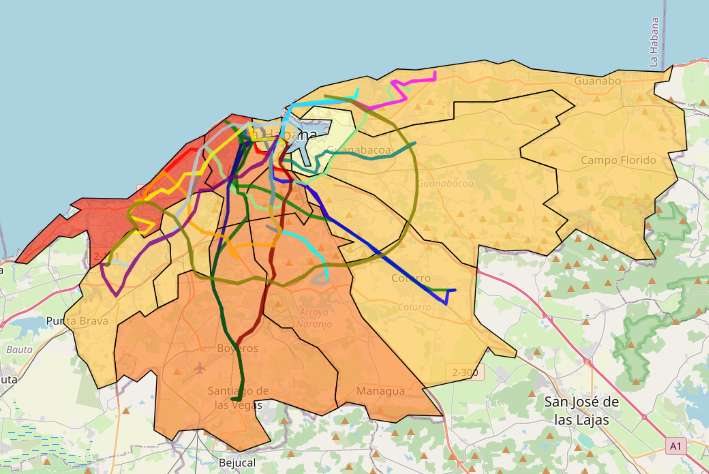
\includegraphics[width=1\textwidth]{imgs/mc.png}
    \caption{Mapa de Calor con el filtro de Rutas visible}
    \label{fig:3}
\end{figure}

An\'alogamente a lo visto en la Figura \ref{fig:2} se presentan dos muestras curiosas de la simulaci\'on, la Figura \ref{fig:4} y la Figura \ref{fig:5}, en la primera se observa una tendencia de los agentes de ir al municipio Plaza de la Revoluci\'on y no regresar, el hecho aqu\'i es que la cantidad de agentes al superar en gran medida a la cantidad de guaguas, estas no puden brindar un buen servicio, por lo que muchos de los agentes en su af\'an de cumplir sus deseos deciden llegar al destino, en su mayor\'ia inclinados m\'as por ir caminando que en carro, por lo cual muchos llegan a sus respectivos empleos bastante tarde, el problema es que al regresar, como simulamos un solo d\'ia ellos llegar\'ian a su casa en su mayor\'ia al d\'ia siguiente, lo cual no se ve reflejado en la gr\'afica. Con respecto a la otra figura notar que pese a la ausencia del P1 como ruta, se mantiene bastante igual el comportamiento a la FIgura \ref{fig:2}, esto se debe al comportamiento del agente de poder encontrar una ruta alternativa a su destino.

\begin{figure}[H]
    \hspace{-3cm}
    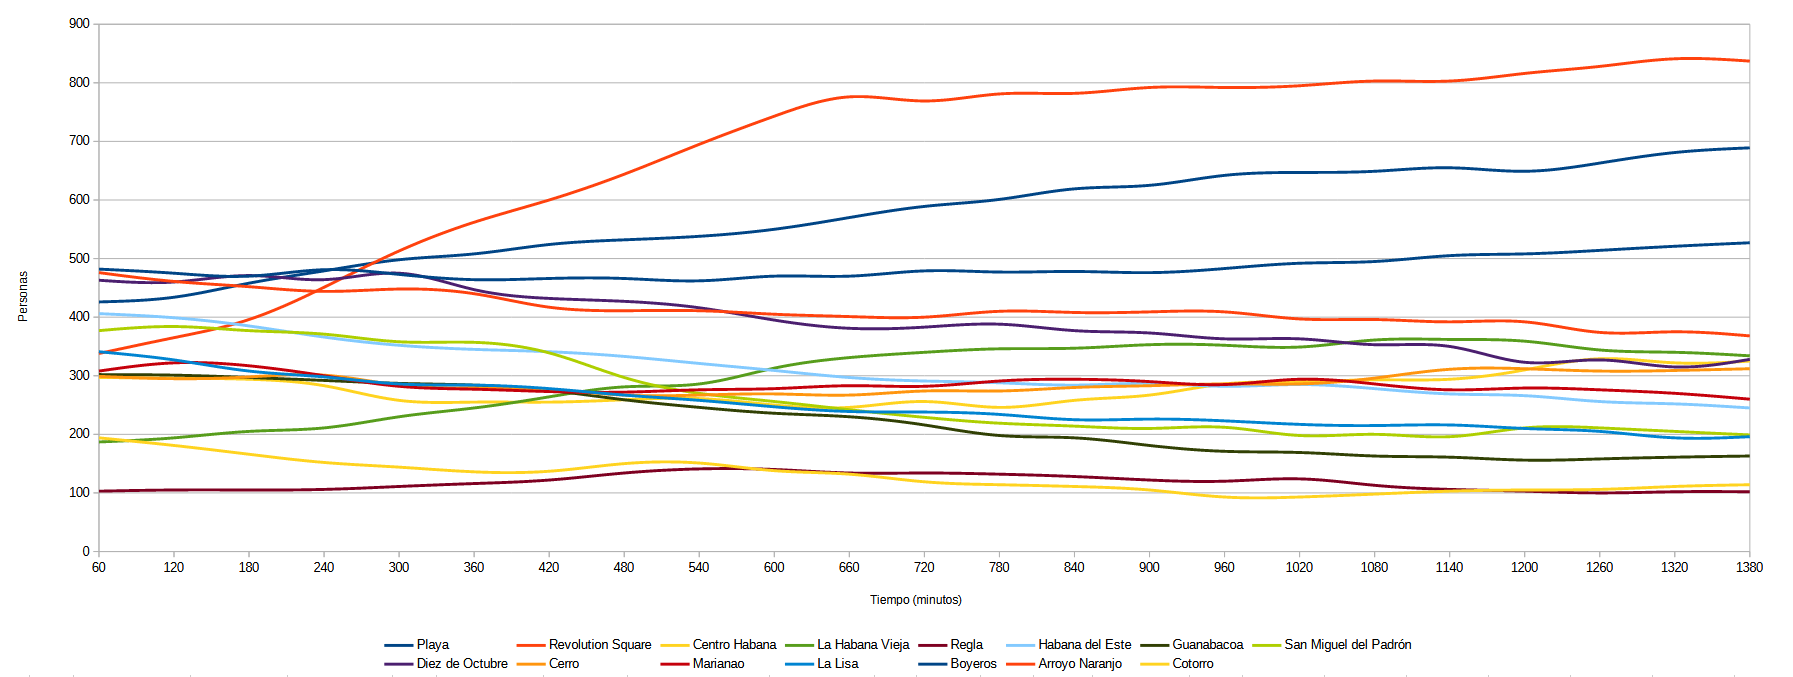
\includegraphics[width=1.4\textwidth]{imgs/s500c2.png}
    \caption{Cantidad de agentes vs Tiempo Minutos (Simulaci\'on 5000 agentes con capacidad de las guaguas de 2, y sin la ausencia de rutas)}
    \label{fig:4}
\end{figure}
\begin{figure}[H]
    \hspace{-3cm}
    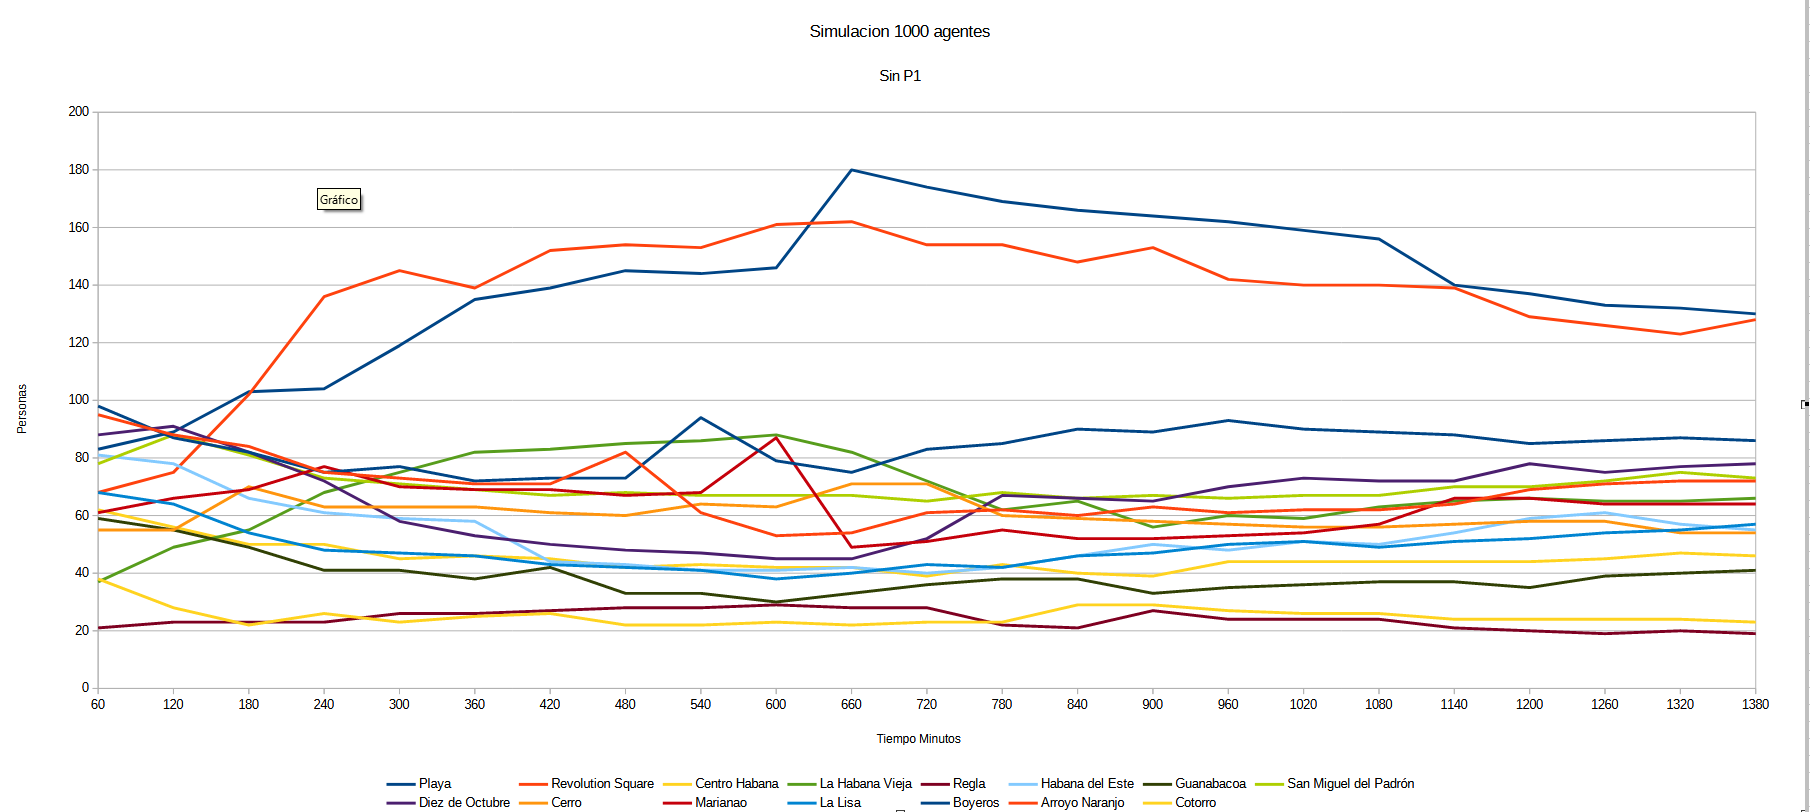
\includegraphics[width=1.4\textwidth]{imgs/s1000c20p1.png}
    \caption{Cantidad de agentes vs Tiempo Minutos (Simulaci\'on 1000 agentes con capacidad de la guagua de 20, y con la ausencia de la ruta P1)}
    \label{fig:5}
\end{figure}

Analizando la muestra de la Figura \ref{fig:5} surge una pregunta: ¿Qué tanto influye entonces una ruta en el desplazamiento de los agentes? Como respuesta veamos lo que sucede en la Figura \ref{fig:6}, en esta se aprecia un alto \'indice de agentes transportados en las rutas que transitan Plaza de la Revoluci\'on y Playa tales como el P9,P1,P2 y PC muy fuertemente ligado a las cuestiones ya mencionadas de tener alta tasa de trabajos. Tal como se observa el n\'umero de personas que usan el transporte p\'ublico es bastante alto, lo cual se considera un se logr\'o pues se acerca m\'as a realidad, teniendo en cuenta que no se us\'o una frecuencia de salida de guaguas muy cerca en el tiempo (60 minutos).

\begin{figure}[H]
     \hspace{-2cm}
    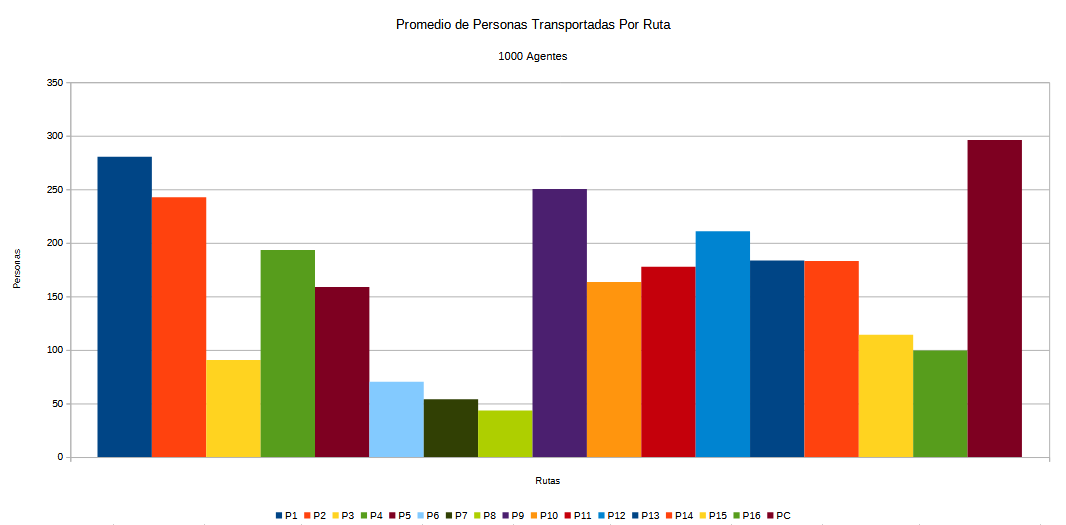
\includegraphics[width=1.3\textwidth]{imgs/pptr.png}
    \caption{Promedio de Personas Transportadas por Ruta}
    \label{fig:6}
\end{figure}
\begin{figure}[H]
    \centering
    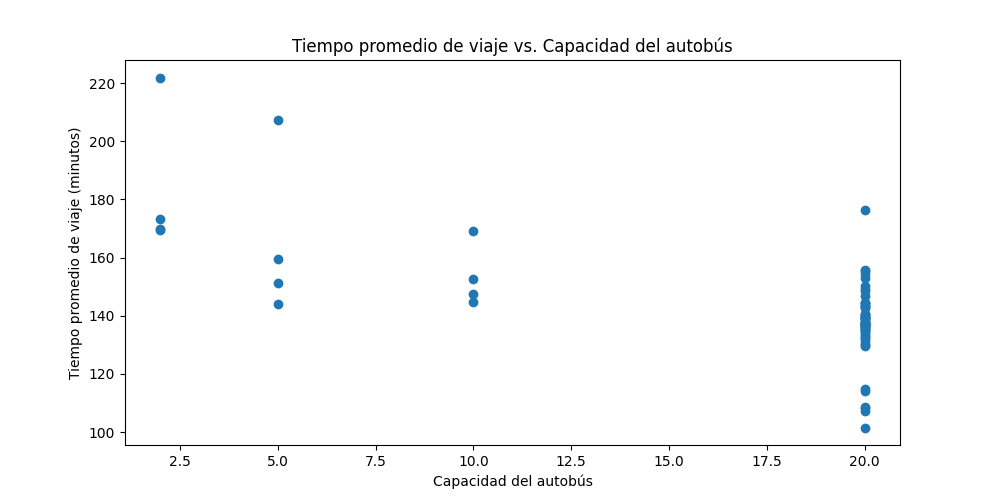
\includegraphics[width=1\textwidth]{imgs/tiempo_capacidad.png}
    \caption{Tiempo Promedio de Viaje(minutos) vs Capacidad del \'omnibus}
    \label{fig:7}
\end{figure}
\newpage
A continuaci\'on vemos en la Figura \ref{fig:7} una correlaci\'on entre el tiempo promedio de viaje y la capacidad de la guaga, indicando que entre m\'as haya capacidad m\'as r\'apido llegan las personas a sus respectivos destinos, aunque notar cierta peculiaridad en que la media de muestras en 20 est\'a ligeramente por encima de la media de las muestras de 10, queda pendiente analizar esto al detalle, puesto que carece un tanto de sentido con la visi\'on puesta en lo real. 


\section{Conclusiones}
Se cumpli\'o el objetivo trazado de poder representar con un enfoque en el transporte p\'ublico la cantidad de personas por municipio en La Habana a lo largo de un d\'ia. Las simulaciones han revelado información interesante sobre el comportamiento del sistema bajo diferentes condiciones. Se ha observado que la demanda de transporte público varía según la zona y la ruta. El tiempo promedio de viaje está correlacionado con la cantidad de agentes y la capacidad del autobús. La capacidad de los autobuses tiene un impacto directo en la cantidad de pasajeros que pueden transportar. Los resultados sugieren que la optimización de estos factores es clave para mejorar el rendimiento del sistema de transporte público. 

\subsection{Recomendaciones}

\begin{itemize}
\item Optimizar las rutas para minimizar el tiempo promedio de viaje y la cantidad de pasajeros que utilizan las rutas con menor demanda.
\item Disminuir el tiempo de salida de guaguas en la rutas P1,P2,P9 y PC ya que según nuestros datos observamos que  se transporta a una cantidad mayor de personas, lo cual reduciría los tiempos de viajes y una mayor cantidad de personas podrían llegar a su objetivo más rápidamente y mejorar la satisfacción de los pasajeros.
\end{itemize}

\subsection{Próximos Pasos}

La simulación podría mejorarse al incluir elementos como:

\begin{itemize}
\item Simulación con los datos reales de población y capacidad de guaguas, así como todas las rutas de estas para un mayor entendimiento del comportamiento de la población de la ciudad de La Habana durante el día.
\item Observaci\'on de las simulaciones mediante la interfaz del mapa implementado vi\'endose las guaguas recorriendo el mapa.
\item Simulaci\'on de las rutas alimentadoras y complementarias como los son la 179,69,A27 entre otras, as\'i como el servicio de Metrotaxi.
\item Con el tema de distancia si se tiene en cuenta donde la guagua dobla se simula mejor los tiempos de llegada de esta a una parada.
\end{itemize}

La implementación de estos elementos permitirá obtener resultados más precisos y útiles para la toma de decisiones en el sistema de transporte público de La Habana.


% Sección de Bibliografía
\bibliographystyle{unsrtnat} % o el estilo que prefieras
\bibliography{bibliography} % Asegúrate de que el archivo .bib está en el mismo directorio


\end{document}
